% Preambel mit Einstellungen importieren
% Document type and used packages
\documentclass[open=right, % Sorgt für Umbruch bei Chapter (any erzeugt keine Leerseiten) -> Kapitel darf nur auf der rechten Seite beginnen
    paper=A4,               % DIN-A4-Papier
    a4paper,                % DIN-A4-Papier
    12pt,                   % Schriftgöße
    headings=small,         % Kleine Überschriften
    headsepline=true,       % Trennlinie am Kopf der Seite
    footsepline=false,      % Keine Trennlinie am Fuß der Seite
    bibliography=totoc,     % Literaturverzeichnis in das Inhaltsverzeichnis aufnehmen
    twoside=off,            % Für doppelseitigen Druck auf on stellen, off für einseitig
    DIV=7,                  % Verhältnis der Ränder zum bedruckten Bereich
    chapterprefix=false,     % Kapitel x vor dem Kapitelnamen
    cleardoublepage=plain]{scrbook}

% Pakete einbinden, die benötigt werden
\usepackage{scrlayer-scrpage}
\usepackage[utf8]{inputenc}       % Dateien in UTF-8 benutzen
\usepackage[T1]{fontenc}          % Zeichenkodierung
\usepackage{graphicx}             % Bilder einbinden
\usepackage[main=ngerman, english]{babel}       % Deutsch und Englisch unterstützen
\usepackage{xcolor}               % Color support
\usepackage{amsmath}              % Matheamtische Formeln
\usepackage{amsfonts}             % Mathematische Zeichensätze
\usepackage{amssymb}              % Mathematische Symbole
\usepackage{float}                % Fließende Objekte (Tabellen, Grafiken etc.)
\usepackage{booktabs}             % Korrekter Tabellensatz
\usepackage[printonlyused, withpage, footnote]{acronym}  % Abkürzungsverzeichnis [nur verwendete Abkürzugen]
\usepackage{makeidx}              % Sachregister
\usepackage{listings}             % Source Code listings
\usepackage{listingsutf8}         % Listings in UTF8
\usepackage[hang,font={sf,footnotesize},labelfont={footnotesize,bf}]{caption} % Beschriftungen
\usepackage[scaled]{helvet}       % Schrift Helvetia laden
\usepackage[absolute]{textpos}	  % Absolute Textpositionen (für Deckblatt)
\usepackage{calc}                 % Berechnung von Positionen
\usepackage{blindtext}            % Blindtexte
\usepackage[bottom=40mm,left=35mm,right=35mm,top=30mm]{geometry} % Ränder ändern
\usepackage{setspace}             % Abstände korrigieren
\usepackage{ifthen}               % Logische Bedingungen mit ifthenelse
\usepackage{scrhack}              % Get rid of tocbasic warnings
\usepackage[pagebackref=false,german]{hyperref}  % Hyperlinks
\usepackage[all]{hypcap}          % Korrekte Verlinkung von Floats
\usepackage[autostyle=true,german=quotes]{csquotes}   % Zitate
\usepackage[backend=biber,
  isbn=true,                     % ISBN nicht anzeigen, gleiches geht mit nahezu allen anderen Feldern
  sortlocale=de_DE,               % Sortierung der Einträge für Deutsch
  %sortlocale=en_US,              % Sortierung der Einträge für Englisch
  autocite=inline,                % regelt Aussehen für \autocite (inline=\parancite)
  hyperref=true,                  % Hyperlinks für Ziate
  %style=ieee                     % Zitate als Zahlen [1]
  %style=alphabetic               % Zitate als Kürzel und Jahr [Ein05]
  %style=authoryear                % Zitate Author und Jahr [Einstein (1905)]
  style=LNI
]{biblatex}                       % Literaturverwaltung mit BibLaTeX
\usepackage{rotating}             % Seiten drehen
\usepackage{harveyballs}          % Harveyballs
\usepackage{tcolorbox}
\usepackage[export]{adjustbox}
\usepackage{subcaption}
\usepackage{color}
\usepackage{colortbl}
\usepackage{wrapfig}
\usepackage{todonotes}
\usepackage{tabularx}
\newcolumntype{b}{>{\hsize=1.2\hsize}X}
\newcolumntype{m}{>{\hsize=.5\hsize}X}
\newcolumntype{s}{>{\hsize=.3\hsize}X}
\usepackage{tikz}


\setlength{\bibitemsep}{1em}     % Abstand zwischen den Literaturangaben
\setlength{\bibhang}{2em}        % Einzug nach jeweils erster Zeile

% Trennung von URLs im Literaturverzeichnis (große Werte [> 10000] verhindern die Trennung)
\defcounter{biburlnumpenalty}{10} % Strafe für Trennung in URL nach Zahl
\defcounter{biburlucpenalty}{500}  % Strafe für Trennung in URL nach Großbuchstaben
\defcounter{biburllcpenalty}{500}  % Strafe für Trennung in URL nach Kleinbuchstaben

% Farben definieren
\definecolor{linkblue}{RGB}{0, 0, 100}
\definecolor{linkblack}{RGB}{0, 0, 0}
\definecolor{comment}{RGB}{63, 127, 95}
\definecolor{darkgreen}{RGB}{14, 144, 102}
\definecolor{darkblue}{RGB}{0,0,168}
\definecolor{darkred}{RGB}{128,0,0}
\definecolor{javadoccomment}{RGB}{0,0,240}
\definecolor{Gray}{RGB}{242,242,242}

% Einstellungen für das Hyperlink-Paket
\hypersetup{
    colorlinks=true,      % Farbige links verwenden
%    allcolors=linkblue,
    linktoc=all,          % Links im Inhaltsverzeichnis
    linkcolor=linkblack,  % Querverweise
    citecolor=linkblack,  % Literaturangaben
	filecolor=linkblack,  % Dateilinks
	urlcolor=linkblack    % URLs
}

% Einstellungen für Quelltexte
\definecolor{backcolour}{rgb}{0.95,0.95,0.92}
\definecolor{codegray}{rgb}{0.5,0.5,0.5}
\lstset{
      xleftmargin=0.1cm,
      basicstyle=\footnotesize\ttfamily,
      keywordstyle=\color{darkgreen},
      identifierstyle=\color{darkblue},
      commentstyle=\color{comment},
      stringstyle=\color{darkred},
      tabsize=2,
      lineskip={2pt},
      columns=flexible,
      inputencoding=utf8,
      captionpos=b,
      backgroundcolor=\color{backcolour},   
      breakautoindent=true,
	  breakindent=2em,
	  breaklines=true,
	  prebreak=,
	  postbreak=,
      numbers=left,                    
      numbersep=5pt,  
      numberstyle=\tiny\color{codegray},  
      showspaces=false,      % Keine Leerzeichensymbole
      showtabs=false,        % Keine Tabsymbole
      showstringspaces=false,% Leerzeichen in Strings
      morecomment=[s][\color{javadoccomment}]{/**}{*/},
      literate={Ö}{{\"O}}1 {Ä}{{\"A}}1 {Ü}{{\"U}}1 {ß}{{\ss}}2 {ü}{{\"u}}1 {ä}{{\"a}}1 {ö}{{\"o}}1
}


\urlstyle{same}

% Einstellungen für Überschriften
\renewcommand*{\chapterformat}{%
  \Large~\thechapter. ~   		% Große Schrift
  \vspace{0.3cm}               	% Abstand zum Titel des Kapitels
}

% Abstände für die Überschriften setzen
\renewcommand{\chapterheadstartvskip}{\vspace*{2.6cm}}
\renewcommand{\chapterheadendvskip}{\vspace*{1.5cm}}

\RedeclareSectionCommand[
  beforeskip=-1.8\baselineskip,
  afterskip=0.25\baselineskip]{section}

\RedeclareSectionCommand[
  beforeskip=-1.8\baselineskip,
  afterskip=0.15\baselineskip]{subsection}

\RedeclareSectionCommand[
  beforeskip=-1.8\baselineskip,
  afterskip=0.15\baselineskip]{subsubsection}


% In der Kopfzeile nur die kurze Kapitelbezeichnung (ohne Kapitel davor)
\renewcommand*\chaptermarkformat{\thechapter\autodot\enskip}
\automark[chapter]{chapter}

% Einstellungen für Schriftarten
\setkomafont{pagehead}{\normalfont\sffamily}
\setkomafont{pagenumber}{\normalfont\sffamily}
\setkomafont{paragraph}{\sffamily\bfseries\small}
\setkomafont{subsubsection}{\sffamily\itshape\bfseries\small}
\addtokomafont{footnote}{\footnotesize}
\setkomafont{chapter}{\LARGE\selectfont\bfseries}

% Wichtige Abstände
\setlength{\parskip}{0.2cm}  % 2mm Abstand zwischen zwei Absätzen
\setlength{\parindent}{0mm}  % Absätze nicht einziehen
\clubpenalty = 10000         % Keine "Schusterjungen"
\widowpenalty = 10000        % Keine "Hurenkinder"
\displaywidowpenalty = 10000 % Keine "Hurenkinder"
\renewcommand{\footnotesize}{\fontsize{9}{10}\selectfont} % Größe der Fußnoten
\setlength{\footnotesep}{8pt} % Abstand zwischen den Fußnoten

% Index erzeugen
\makeindex

% Einfacher Font-Wechsel über dieses Makro
\newcommand{\changefont}[3]{
\fontfamily{#1} \fontseries{#2} \fontshape{#3} \selectfont}

% Eigenes Makro für Bilder
\newcommand{\bild}[3]{
\begin{figure}[h]
  \centering
  \includegraphics[width=#2]{#1}
  \caption{#3}
  \label{#1}
\end{figure}}

% Wo liegt Sourcecode?
\newcommand{\srcloc}{src/}

% Wo sind die Bilder?
\graphicspath{{bilder/}}

% Makros für typographisch korrekte Abkürzungen
\newcommand{\zb}[0]{z.\,B.\ }
\newcommand{\dahe}[0]{d.\,h.\ }
\newcommand{\ua}[0]{u.\,a.\ }

% Flags für Veröffentlichung und Sperrvermerk
\newboolean{hsmapublizieren}
\newboolean{hsmasperrvermerk}


% Dokumenteninfos importieren
% In docinfo.tex sind Titel, Autor, Abstract zu definieren
% -------------------------------------------------------
% Daten für die Arbeit
% Wenn hier alles korrekt eingetragen wurde, wird das Titelblatt
% automatisch generiert. D.h. die Datei titelblatt.tex muss nicht mehr
% angepasst werden.

% Titel der Arbeit auf Deutsch
\newcommand{\hsmatitelde}{Distributed Denial of Service}

% Weitere Informationen zur Arbeit
\newcommand{\hsmaort}{Offenburg}    % Ort
\newcommand{\hsmaautorvname}{Jonas} % Vorname(n)
\newcommand{\hsmaautornname}{Kienzle} % Nachname(n)
\newcommand{\hsmadatum}{07.08.2020} % Datum der Abgabe
\newcommand{\hsmajahr}{2020} % Jahr der Abgabe
\newcommand{\hsmafirma}{XYZ} % Firma bei der die Arbeit durchgeführt wurde
\newcommand{\hsmabetreuer}{Prof. Dr. rer. nat. Stephan Trahasch, Hochschule Offenburg} % Betreuer an der Hochschule
\newcommand{\hsmafakultaet}{EMI} % Fakultät
\newcommand{\hsmastudiengang}{AI} % Studiengangsabkürzung. 

% -------------------------------------------------------
% Abstract

% Kurze (maximal halbseitige) Beschreibung, worum es in der Arbeit geht auf Deutsch
\newcommand{\hsmaabstractde}{DDoS-Angriffe werden in der heutigen Zeit zu einem immer größeren Problem. Mit der immer weiterschreitenden Digitalisierung entstehen täglich neue potenzielle Geräte, welche zum Angriff verwendet werden können. Gleichermaßen wächst auf der Seite der Software auch immer die Angriffsfläche und somit die Zahl der möglichen Einfallstore für diese Art von Angriffen. Im Folgenden wird ein Überblick über DoS- und DDoS-Attacken im Allgemeinen gegeben. Ebenfalls werden mögliche Angriffsmethoden wie zum Beispiel HTTP Slow Post oder SYN-Flooding vorgestellt. Schließlich werden noch ein paar der möglichen Schutzmaßnahmen aufgezeigt.}


% Literatur-Datenbank
\addbibresource{literatur.bib}   % BibLaTeX-Datei mit Literaturquellen einbinden

\begin{document}
\frontmatter

% Römische Ziffern für die "Front-Matter"
\setcounter{page}{0}
\changefont{ptm}{m}{n}  % Times New Roman für den Fließtext
\renewcommand{\rmdefault}{ptm}

% Titelblatt
% -------------------------------------------------------
% In dieser Datei sollten eigentlich keine Veränderungen mehr
% notwendig sein.
% -------------------------------------------------------

\thispagestyle{empty}

% Fakultät
% -------------------------------------------------------
\newcommand{\hsmafakultaetlangde}{Fakultät Elektrotechnik, Medizintechnik und Informatik}

\newcommand{\hsmastudienganglangde}{Angewandte Informatik}
\newcommand{\hsmatypde}{HAUSARBEIT}

\newcommand{\hsmakoerperschaftde}{Hochschule für Technik, Wirtschaft und Medien Offenburg}

\newcommand{\hsmaautorbib}{Jonas Kienzle und Hannes Braun} % Autor Nachname, Vorname
\newcommand{\hsmaautor}{Jonas Kienzle und Hannes Braun} % Autor Vorname Nachname


\newcommand{\hsmatyp}{\hsmatypde}%
\newcommand{\hsmathesistype}{Praktikum IT-Security}%
\newcommand{\hsmakoerperschaft}{\hsmakoerperschaftde}%
\newcommand{\hsmastudiengangname}{Studiengang \hsmastudienganglangde}%
\newcommand{\hsmastudienganglang}{\hsmastudienganglangde}%
\newcommand{\hsmatitel}{\hsmatitelde}%
\newcommand{\hsmatutor}{Dozent}%
\newcommand{\hsmafakultaetlang}{\hsmafakultaetlangde}%
\newcommand{\hsmalistoftables}{Tabellenverzeichnis}%
\newcommand{\hsmalistoffigures}{Abbildungsverzeichnis}%
\newcommand{\hsmalistings}{Quellcodeverzeichnis}%
\newcommand{\hsmaindex}{Index}%
\newcommand{\hsmaabbreviations}{Abkürzungsverzeichnis}%   
\selectlanguage{ngerman}


% Daten in die Standard-Felder von KOMA-Script eintragen
\titlehead{\hsmatyp\ in\  \hsmastudienganglang}
\subject{}
\title{\hsmatitel}
\author{\hsmaauthor}
\date{\small{\hsmadatum}}

% Daten für das fertige PDF-Dokument
\hypersetup{
  pdftitle={\hsmatitel},  % Titel des Dokuments
  pdfauthor={\hsmaautor},              % Autor
  pdfsubject={\hsmatyp\ in\ \hsmastudienganglang},                % Thema
  pdfkeywords={\hsmatitel}         % Schlüsselworte
}

\newlength{\bindekorrektur}
\newlength{\seitenanfang}
\newlength{\seitenbreite}
  
\setlength{\bindekorrektur}{-46mm}   % Korrektur der horizontalen Position
\setlength{\seitenanfang}{0mm}       % Korrektur der vertikalen Position
\setlength{\seitenbreite}{297mm}

%\noindent 
\includegraphics[width=7cm, left]{hso.png}\hfill 
\includegraphics[width=2cm, right]{edeka.png} \\
\captionsetup[figure]{labelformat=empty}
\noindent 
\begin{figure}
  
\includegraphics[width=10cm,center]{hso.jpg}
  \caption[]{}
\end{figure}
\captionsetup[figure]{labelformat=simple}
% Titel der Arbeit
\begin{textblock*}{128mm}(41mm,\seitenanfang + 62mm) % 4,5cm vom linken Rand und 6,0cm vom oberen Rand
  \centering\Large\sffamily
  \vspace{12mm} % Kleiner zusätzlicher Abstand oben für bessere Optik
  \textbf{\hsmatitel}
\end{textblock*}%

% Name
\begin{textblock*}{\seitenbreite}(\bindekorrektur,\seitenanfang + 108mm)
  \centering\large\sffamily
  \hsmaautor
\end{textblock*}

% Thesis
\begin{textblock*}{\seitenbreite}(\bindekorrektur,\seitenanfang + 130mm)
  \centering\large\sffamily
  \textbf{\hsmatyp}\\
  \begin{small}\hsmathesistype \end{small}\\
  \vspace{6mm}
  \hsmastudiengangname
\end{textblock*}

% Fakultät
\begin{textblock*}{\seitenbreite}(\bindekorrektur,\seitenanfang + 165mm)
  \centering\large\sffamily
  \hsmafakultaetlang\\
  \vspace{2mm}
  \hsmakoerperschaft
\end{textblock*}

% Datum
\begin{textblock*}{\seitenbreite}(\bindekorrektur,\seitenanfang + 190mm)
  \centering\large 
  \textsf{\hsmadatum}
\end{textblock*}

% Betreuer
\begin{textblock*}{\seitenbreite}(\bindekorrektur,\seitenanfang + 240mm)
  \centering\large\sffamily
  \hsmatutor \\
  \vspace{2mm}
  \hsmabetreuer\\
\end{textblock*}

\cleardoublepage

% Abstract
\thispagestyle{empty}
\textsf{\large\textbf{Zusammenfassung}}
\subsubsection*{\hsmatitelde}\hsmaabstractde



% Inhaltsverzeichnis erzeugen
\cleardoublepage
\pdfbookmark{\contentsname}{Contents}
\tableofcontents

% Korrigiert Nummerierung bei mehrseitigem Inhaltsverzeichnis
\cleardoublepage
\newcounter{frontmatterpage}
\setcounter{frontmatterpage}{\value{page}}

% Arabische Zahlen für den Hauptteil
\mainmatter

% Den Hauptteil mit vergrößertem Zeilenabstand setzen
\onehalfspacing

% ------------------------------------------------------------------
% Hauptteil der Arbeit
\chapter{Was ist ein DDoS-Angriff?}
\label{chap:kapitel1}
Die Grundlage für einen \ac{ddos}-Angriff ist ein \ac{dos}-Angriff. Ein \ac{dos}-Angriff (Denial-of-Service-Angriff) hat das Ziel ein System nicht mehr verfügbar zu machen. Dazu kann entweder die begrenzte Bandbreite so ausgenutzt werden, dass die eigentlichen Nutzer des Systems dieses nicht mehr erreichen können. Eine andere Möglichkeit ist die Überlastung des Systems selbst (CPU, RAM, ...), damit dieses nicht mehr (zeitnah) antworten kann.

Solche Angriffe richten meist keinen permanenten Schaden an der IT-Infrastruktur direkt an. Ist der Angriff vorbei, so kann der Normalbetrieb in der Regel wieder aufgenommen werden. Dennoch können sie einen (erheblichen) finanziellen Schaden anrichten. Das gilt beispielsweise für Unternehmen, welche sehr stark auf den Verkauf ihrer Waren im Internet setzen. Eine Nichtverfügbarkeit würde hierbei enorme finanzielle Einbuße einbringen. Auf diese Weise werden diese Unternehmen bei einem schlechten Schutz gegen solche Angriffe auch relativ schnell erpressbar.

Eine Unterkategorie dieser Angriffe ist der \acl{ddos}-Angriff. Dieser unterscheidet sich dadurch, dass hierbei der Ursprung des Angriffs explizit nicht nur von einem Computer aus kommt, sondern von einer Vielzahl von Computern. Für diese Realisierung wird oftmals ein Botnetz verwendet. Ein Botnetz ist eine Menge aus Computern, welche meist ohne das Wissen des Besitzers unter der Kontrolle eines Angreifers stehen. Dazwischen steht in der Regel noch ein Command-and-Control-Server. Dieser nimmt die Befehle des Angreifers entgegen und kommuniziert diese weiter an die Bots.

\begin{figure}[h]
		\centering
		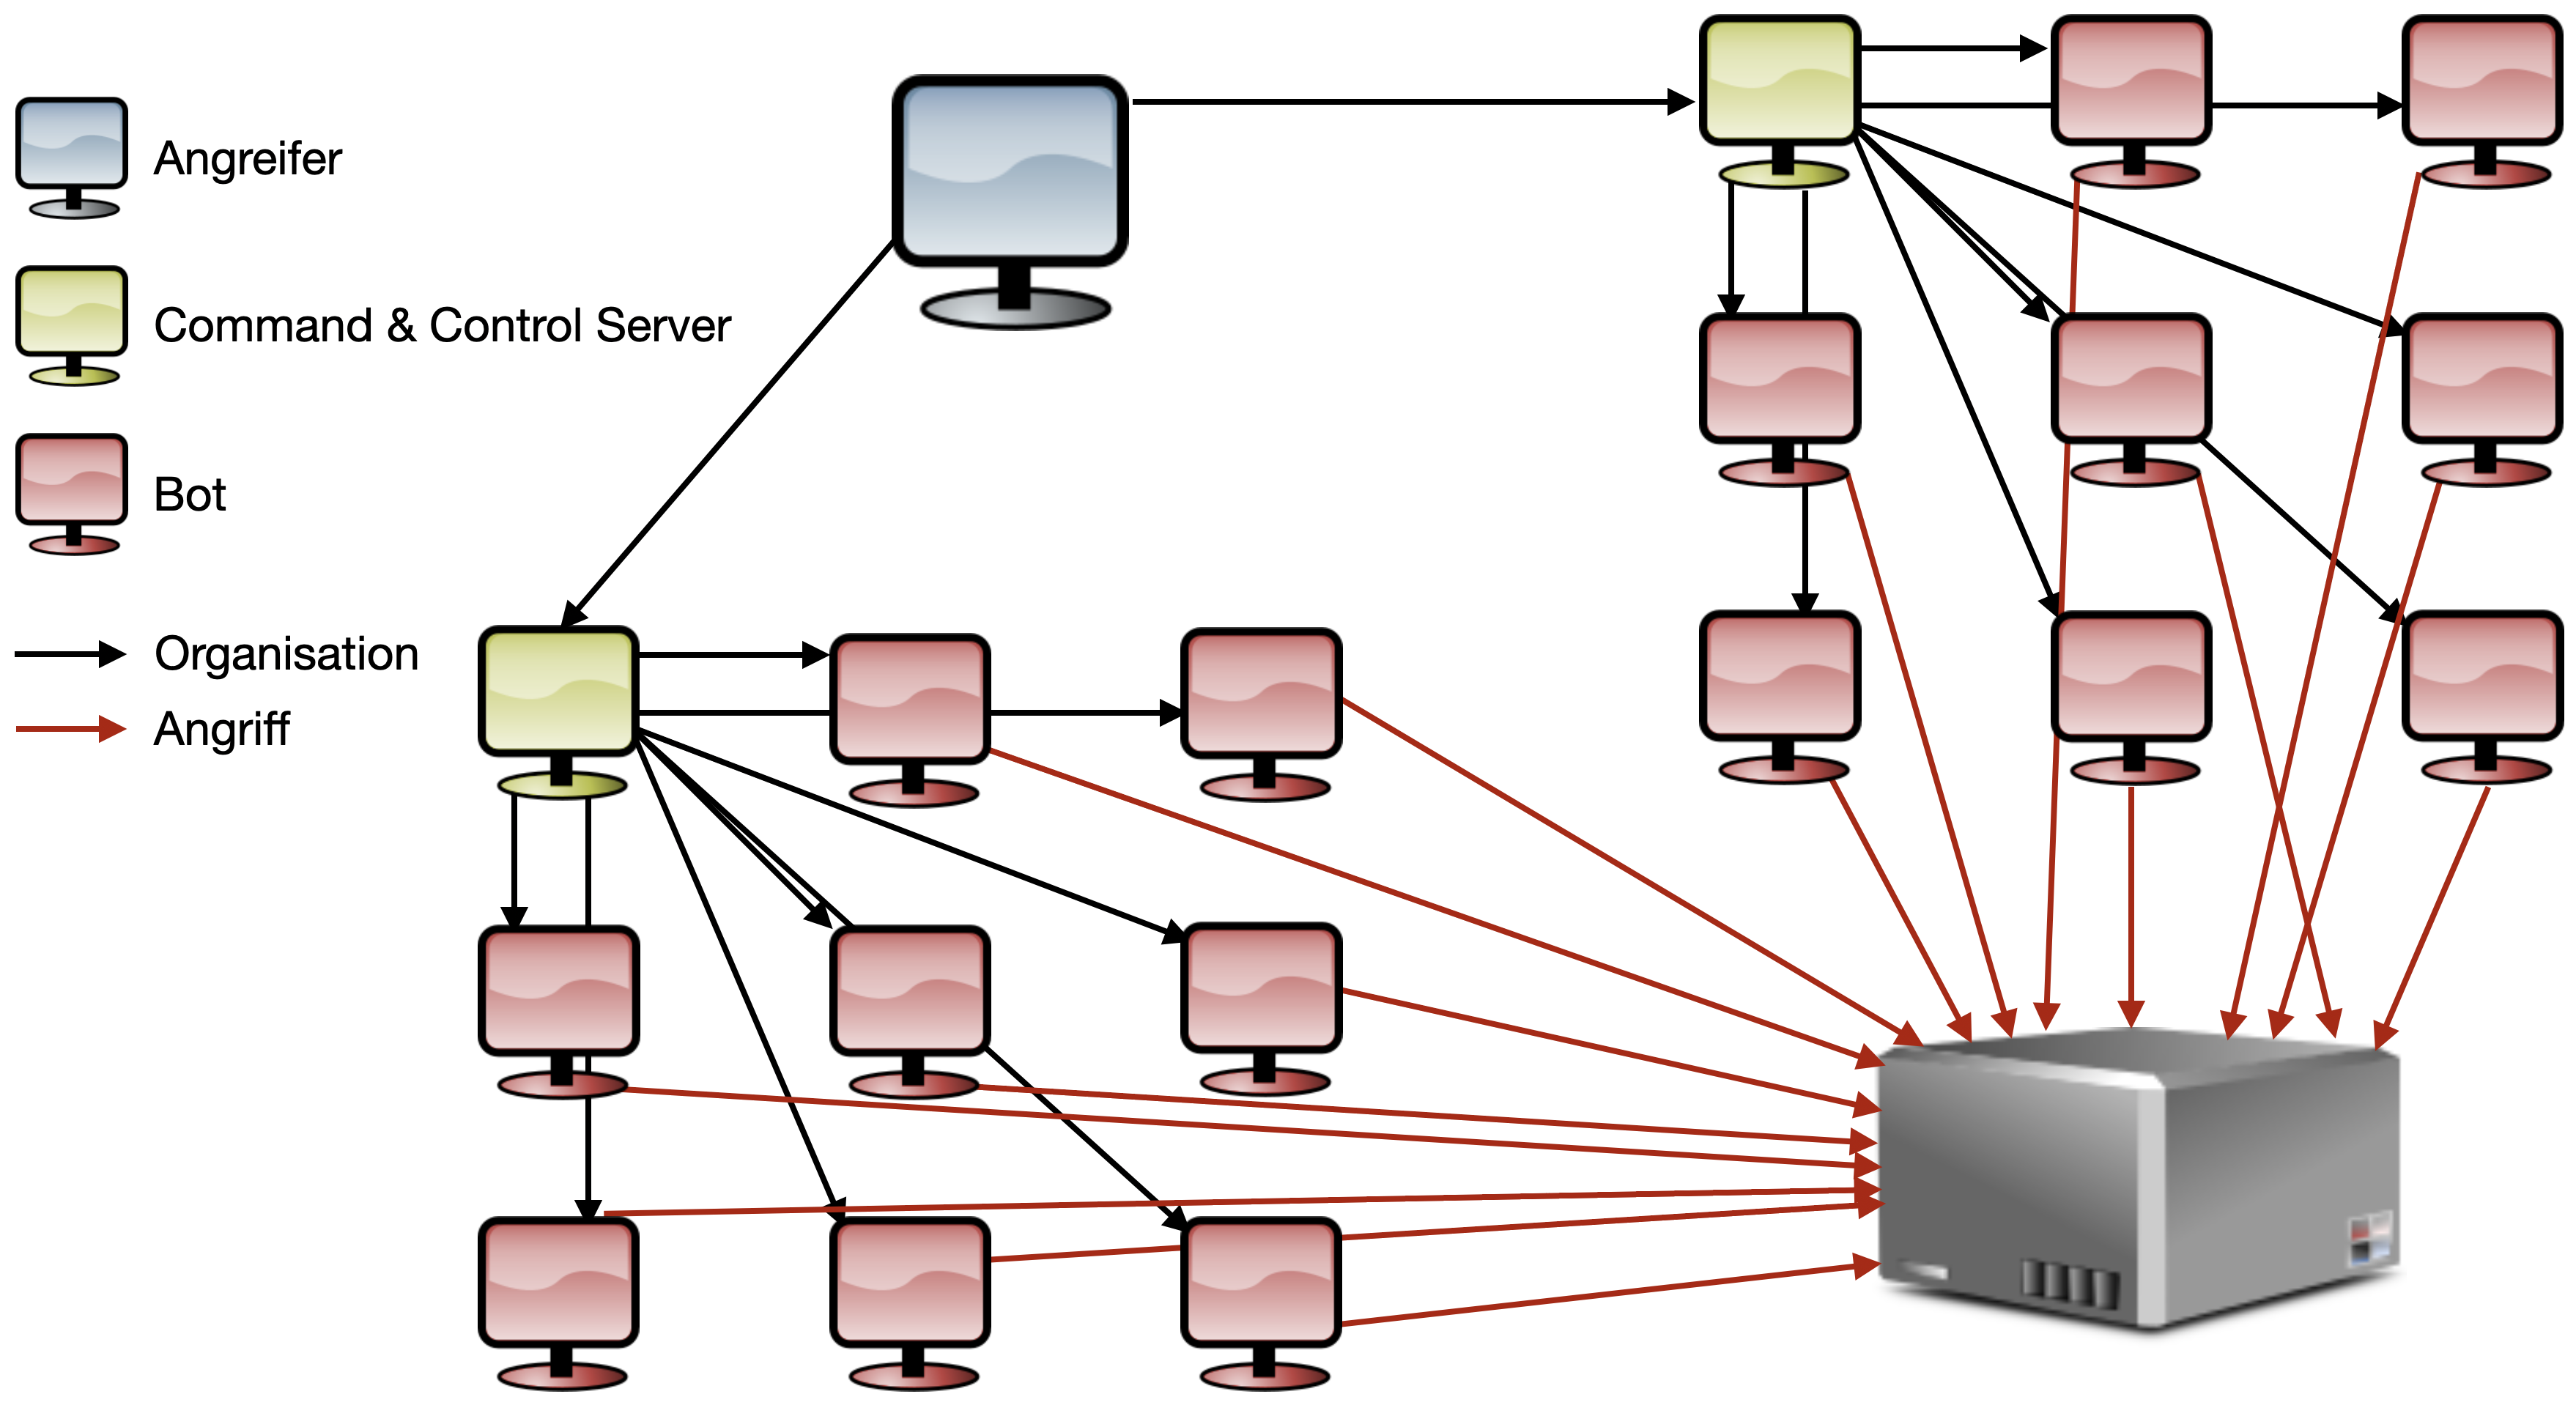
\includegraphics[width=\textwidth, center]{kapitel1/botnet}
		\caption[Schematischer Aufbau bei einem DDoS-Angriff mit einem Botnetz]{Schematischer Aufbau eines Botnetzes zur Durchführung eines DDoS-Angriffs}
		\label{img:botnet}
\end{figure}

Eine Analogie zu einem DDoS-Angriff aus dem realen Leben wäre die Benutzung von einem Bus. Spricht man sich hierbei ab, dass sehr viele Leute gleichzeitig versuchen in einen Bus einzusteigen, so bleibt kaum bis kein Platz mehr für die eigentlichen Fahrgäste. Das Ergebnis ist die Nichtverfügbarkeit eines Systems, in diesem Fall der Bus.

\chapter{Kapitel 2}
\label{chap:kapitel2}
Eine Abkürzung \ac{cd}, \ac{ci}. Ausgeschrieben \acl{cd}. Verweis zu einem File-Listing \ref{lst:crypter} oder einem Listing im Textfluss \ref{lst:Rggplot} und ein Inline-Listing \lstinline|print("Hello World")|.

\lstinputlisting[language=Java,caption={Ein Listing},label=lst:crypter]{\srcloc/Crypter.java}

\begin{lstlisting}[language=R,caption=Beispielaufruf ldply-Funktion in R, label=lst:Rggplot]
ggplot(data = data, mapping = aes(x=timestamp, y=score) + geom_line()
\end{lstlisting}
			
\chapter{Schutzmaßnahmen}
\label{chap:kapitel3}
Eine Abkürzung \ac{cd}, \ac{ci}. Ausgeschrieben \acl{cd}. Verweis zu einem File-Listing \ref{lst:crypter} oder einem Listing im Textfluss \ref{lst:Rggplot} und ein Inline-Listing \lstinline|print("Hello World")|.

\lstinputlisting[language=Java,caption={Ein Listing},label=lst:crypter]{\srcloc/Crypter.java}

\begin{lstlisting}[language=R,caption=Beispielaufruf ldply-Funktion in R, label=lst:Rggplot]
ggplot(data = data, mapping = aes(x=timestamp, y=score) + geom_line()
\end{lstlisting}
			
% ------------------------------------------------------------------

\label{lastpage}

% Neue Seite
% \clearpage

% Backmatter mit normalem Zeilenabstand setzen
%\singlespacing

% Römische Ziffern für die "Back-Matter", fortlaufend mit "Front-Matter"
\pagenumbering{roman}
%\setcounter{page}{\value{frontmatterpage}}
\setcounter{page}{0}

% Literaturverzeichnis erzeugen
\begin{flushleft}
\printbibliography
\end{flushleft}

% Index ausgeben. Wenn Sie keinen Index haben, entfernen Sie einfach
% diesen Teil.
%\cleardoublepage
%\phantomsection
%\addcontentsline{toc}{chapter}{\hsmaindex}
%\printindex

\end{document}
